\chapter*{A: MVA control plots}

\section*{Hadronic decay MVA training}\label{sec:hadronic-decay-mva-training}

\subsection*{Variable importance}

\begin{longtable}{| p{.05\textwidth} | p{.6\textwidth} | p{.05\textwidth} |p{.2\textwidth} |}
\hline
& Name & Alias & Importance \\ \hline
0 &\texttt{B\_qpKinLepton} & $v_{0}$ & $0.510$ \\ \hline
1 &\texttt{B\_qpIntermediateKinLepton} & $v_{1}$ & $0.170$ \\ \hline
2 &\texttt{B\_nLepInROE} & $v_{2}$ & $0.151$ \\ \hline
3 &\texttt{B\_qpIntermediateElectron} & $v_{3}$ & $0.031$ \\ \hline
4 &\texttt{B\_qpMuon} & $v_{4}$ & $0.026$ \\ \hline
5 &\texttt{B\_ROE\_PThetacms0} & $v_{5}$ & $0.020$ \\ \hline
6 &\texttt{B\_nROEDistTrk} & $v_{6}$ & $0.020$ \\ \hline
7 &\texttt{B\_qpElectron} & $v_{7}$ & $0.019$ \\ \hline
8 &\texttt{B\_ROECharge0} & $v_{8}$ & $0.018$ \\ \hline
9 &\texttt{B\_qpIntermediateMuon} & $v_{9}$ & $0.013$ \\ \hline
10 &\texttt{B\_nROETrk0} & $v_{10}$ & $0.010$ \\ \hline
11 &\texttt{B\_TagVPvalue} & $v_{11}$ & $0.007$ \\ \hline
12 &\texttt{B\_nKaonInROE} & $v_{12}$ & $0.004$ \\ \hline
\captionsetup{width=0.8\linewidth}
\caption{Variable names, aliases and importance in the scope of hadronic decay MVA training.}
\end{longtable}

\subsection*{Variable distributions}

\begin{figure}[H]
\centering
\captionsetup{width=0.8\linewidth}
\subfigure{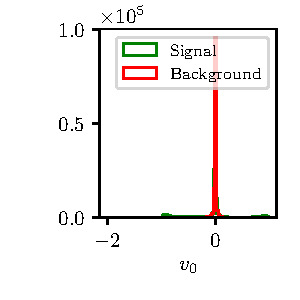
\includegraphics[width=0.241\linewidth]{fig/addendums/HD_v0}}
\subfigure{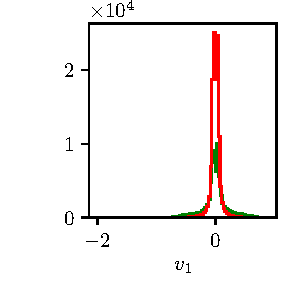
\includegraphics[width=0.241\linewidth]{fig/addendums/HD_v1}}
\subfigure{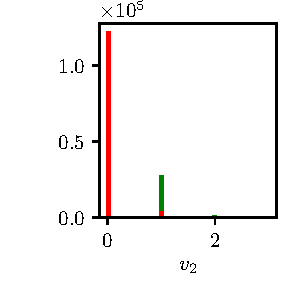
\includegraphics[width=0.241\linewidth]{fig/addendums/HD_v2}}
\subfigure{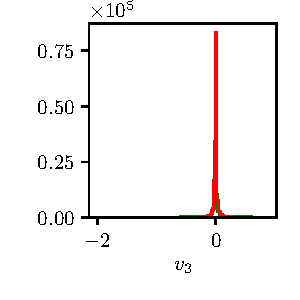
\includegraphics[width=0.241\linewidth]{fig/addendums/HD_v3}}\\
\subfigure{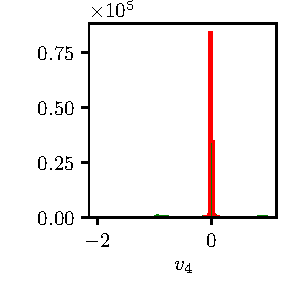
\includegraphics[width=0.241\linewidth]{fig/addendums/HD_v4}}
\subfigure{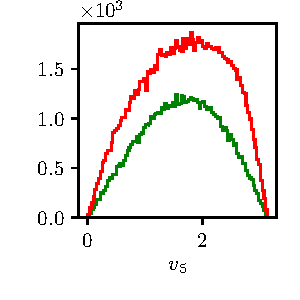
\includegraphics[width=0.241\linewidth]{fig/addendums/HD_v5}}
\subfigure{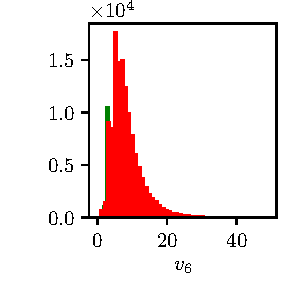
\includegraphics[width=0.241\linewidth]{fig/addendums/HD_v6}}
\subfigure{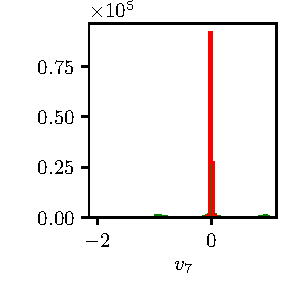
\includegraphics[width=0.241\linewidth]{fig/addendums/HD_v7}}\\
\subfigure{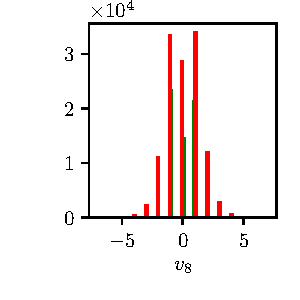
\includegraphics[width=0.241\linewidth]{fig/addendums/HD_v8}}
\subfigure{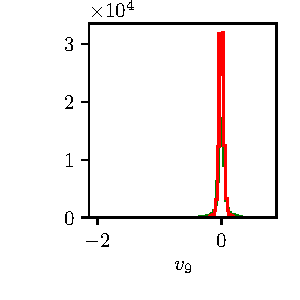
\includegraphics[width=0.241\linewidth]{fig/addendums/HD_v9}}
\subfigure{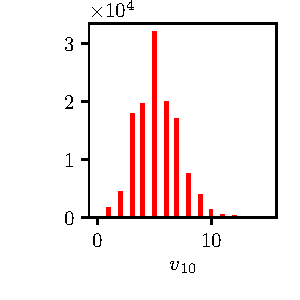
\includegraphics[width=0.241\linewidth]{fig/addendums/HD_v10}}
\subfigure{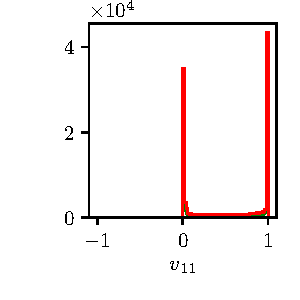
\includegraphics[width=0.241\linewidth]{fig/addendums/HD_v11}}\\
\subfigure{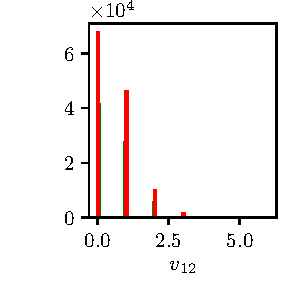
\includegraphics[width=0.241\linewidth]{fig/addendums/HD_v12}}
\caption{Feature distributions for MVA training of hadronically decayed candidates.}
\end{figure}

\subsection*{Hyper-parameter optimization}

\begin{figure}[H]
\centering
\captionsetup{width=0.8\linewidth}
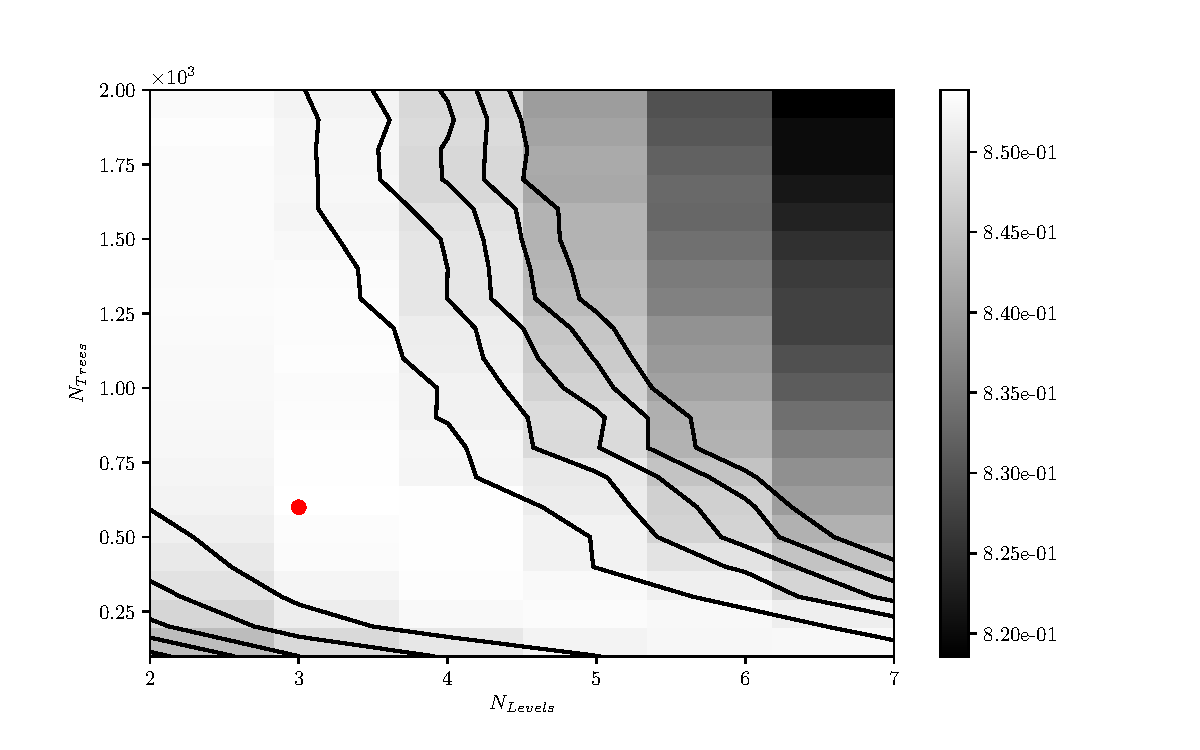
\includegraphics[width=\linewidth]{fig/addendums/HD_hpo}
\caption{Hyper-parameter optimization of \texttt{nTrees} and \texttt{nLevels} in the BDT forest training of hadronically decayed candidates.}
\end{figure}

\subsection*{Results}

\begin{figure}[H]
\centering
\captionsetup{width=0.8\linewidth}
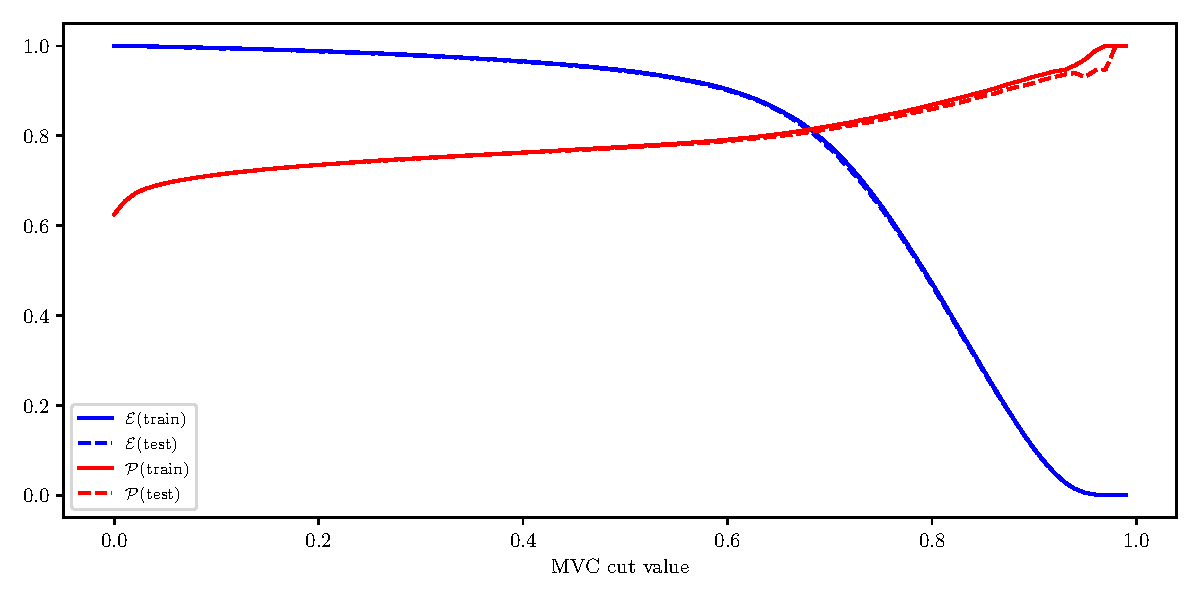
\includegraphics[width=\linewidth]{fig/addendums/HD_effpur}
\caption{Efficiency ($\mathcal{E}$) and purity ($\mathcal{P}$) of the MVA classifier output for hadronically decayed candidates training on the train (solid) and test (dashed) samples.}
\end{figure}

\begin{figure}[H]
\centering
\captionsetup{width=0.8\linewidth}
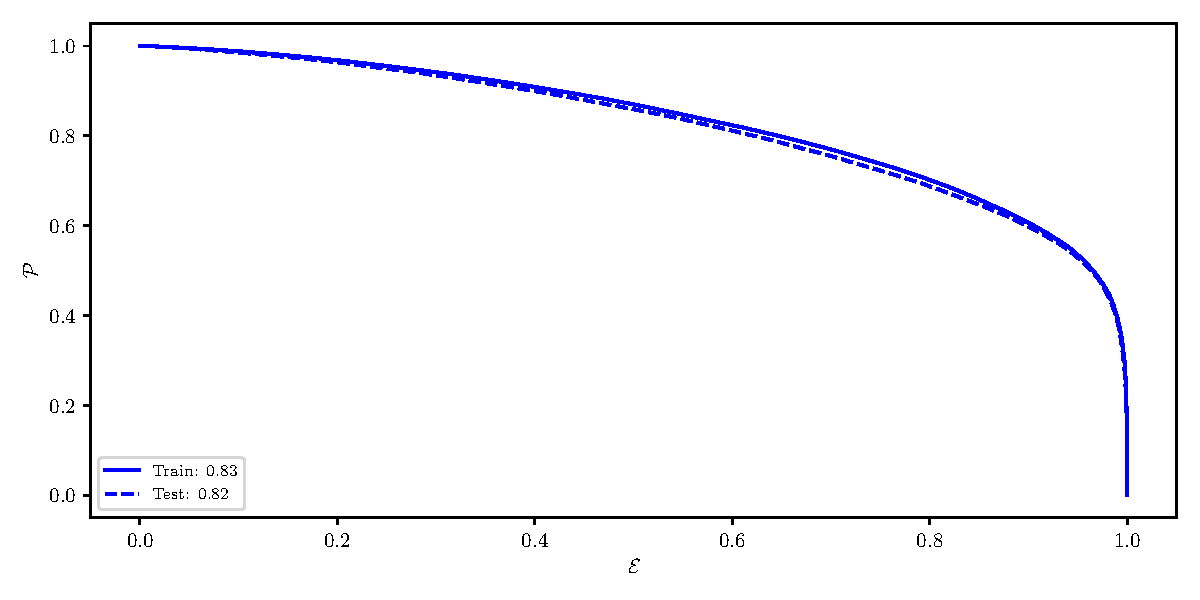
\includegraphics[width=\linewidth]{fig/addendums/HD_roc}
\caption{ROC curves of the MVA classifier output for hadronically decayed candidates training on the train (solid) and test (dashed) samples.}
\end{figure}

\section*{ROE clean-up $\pi^0$ training}\label{sec:ROE_pi0}

\subsection*{Variable importance}

\begin{longtable}{| p{.05\textwidth} | p{.6\textwidth} | p{.05\textwidth} |p{.2\textwidth} |}
\hline
& Name & Alias & Importance \\ \hline
0 &\texttt{chiProb} & $v_{0}$ & $0.262$ \\ \hline
1 &\texttt{useCMSFrame(daughterAngleInBetween(0,1))} & $v_{1}$ & $0.148$ \\ \hline
2 &\texttt{daughter(0,useCMSFrame(p))} & $v_{2}$ & $0.079$ \\ \hline
3 &\texttt{InvM} & $v_{3}$ & $0.076$ \\ \hline
4 &\texttt{daughter(1,clusterHighestE)} & $v_{4}$ & $0.062$ \\ \hline
5 &\texttt{daughter(1,p)} & $v_{5}$ & $0.050$ \\ \hline
6 &\texttt{daughter(1,clusterTheta)} & $v_{6}$ & $0.048$ \\ \hline
7 &\texttt{daughter(0,clusterHighestE)} & $v_{7}$ & $0.031$ \\ \hline
8 &\texttt{daughter(0,clusterTheta)} & $v_{8}$ & $0.028$ \\ \hline
9 &\texttt{daughter(0,minC2HDist)} & $v_{9}$ & $0.023$ \\ \hline
10 &\texttt{daughter(1,minC2HDist)} & $v_{10}$ & $0.021$ \\ \hline
11 &\texttt{daughter(0,clusterE9E25)} & $v_{11}$ & $0.021$ \\ \hline
12 &\texttt{daughter(1,clusterE9E25)} & $v_{12}$ & $0.021$ \\ \hline
13 &\texttt{useRestFrame(daughterAngleInBetween(0,1))} & $v_{13}$ & $0.018$ \\ \hline
14 &\texttt{daughter(1,clusterNHits)} & $v_{14}$ & $0.013$ \\ \hline
15 &\texttt{SigMBF} & $v_{15}$ & $0.013$ \\ \hline
16 &\texttt{daughter(0,clusterNHits)} & $v_{16}$ & $0.013$ \\ \hline
17 &\texttt{useCMSFrame(p)} & $v_{17}$ & $0.012$ \\ \hline
18 &\texttt{daughter(0,clusterErrorE)} & $v_{18}$ & $0.011$ \\ \hline
19 &\texttt{useLabFrame(daughterAngleInBetween(0,1))} & $v_{19}$ & $0.010$ \\ \hline
20 &\texttt{daughter(1,clusterErrorE)} & $v_{20}$ & $0.010$ \\ \hline
21 &\texttt{daughter(1,useCMSFrame(p))} & $v_{21}$ & $0.008$ \\ \hline
22 &\texttt{daughter(0,p)} & $v_{22}$ & $0.007$ \\ \hline
23 &\texttt{p} & $v_{23}$ & $0.007$ \\ \hline
24 &\texttt{SigM} & $v_{24}$ & $0.007$ \\ \hline
\captionsetup{width=0.8\linewidth}
\caption{Variable names, aliases and importance in the scope of $\pi^0$ MVA training for ROE clean-up.}
\end{longtable}

\subsection*{Variable distributions}

\begin{figure}[H]
\centering
\captionsetup{width=0.8\linewidth}
\subfigure{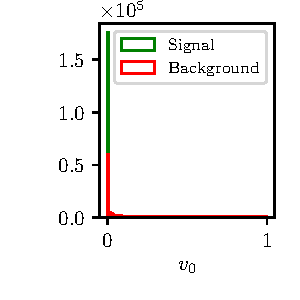
\includegraphics[width=0.241\linewidth]{fig/addendums/pi0_v0}}
\subfigure{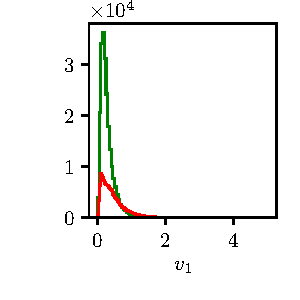
\includegraphics[width=0.241\linewidth]{fig/addendums/pi0_v1}}
\subfigure{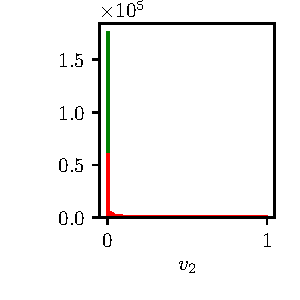
\includegraphics[width=0.241\linewidth]{fig/addendums/pi0_v2}}
\subfigure{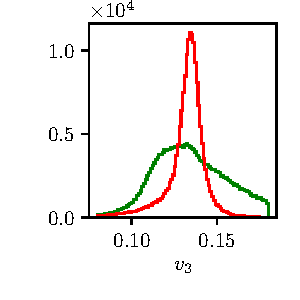
\includegraphics[width=0.241\linewidth]{fig/addendums/pi0_v3}}\\
\subfigure{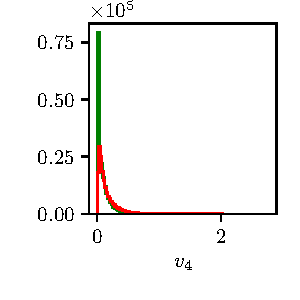
\includegraphics[width=0.241\linewidth]{fig/addendums/pi0_v4}}
\subfigure{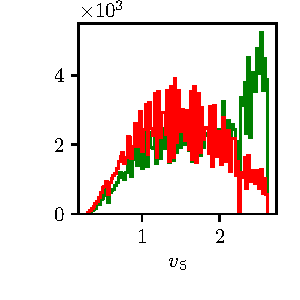
\includegraphics[width=0.241\linewidth]{fig/addendums/pi0_v5}}
\subfigure{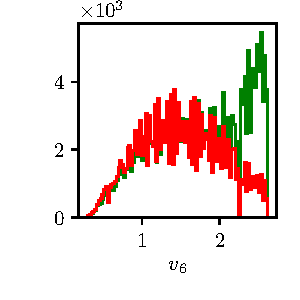
\includegraphics[width=0.241\linewidth]{fig/addendums/pi0_v6}}
\subfigure{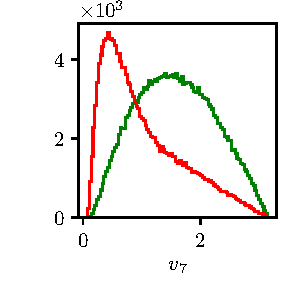
\includegraphics[width=0.241\linewidth]{fig/addendums/pi0_v7}}\\
\subfigure{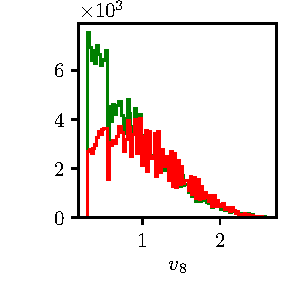
\includegraphics[width=0.241\linewidth]{fig/addendums/pi0_v8}}
\subfigure{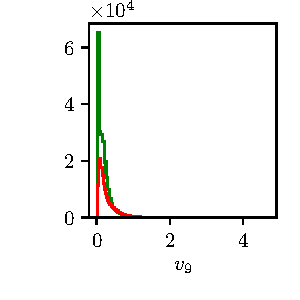
\includegraphics[width=0.241\linewidth]{fig/addendums/pi0_v9}}
\subfigure{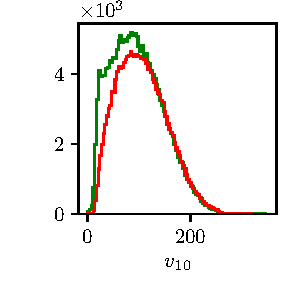
\includegraphics[width=0.241\linewidth]{fig/addendums/pi0_v10}}
\subfigure{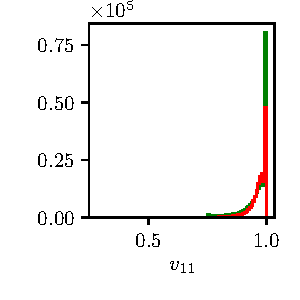
\includegraphics[width=0.241\linewidth]{fig/addendums/pi0_v11}}\\
\subfigure{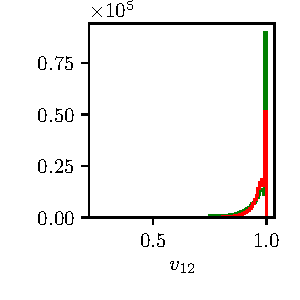
\includegraphics[width=0.241\linewidth]{fig/addendums/pi0_v12}}
\subfigure{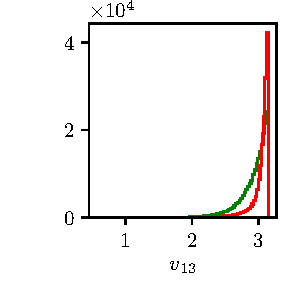
\includegraphics[width=0.241\linewidth]{fig/addendums/pi0_v13}}
\subfigure{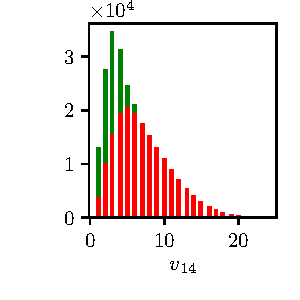
\includegraphics[width=0.241\linewidth]{fig/addendums/pi0_v14}}
\subfigure{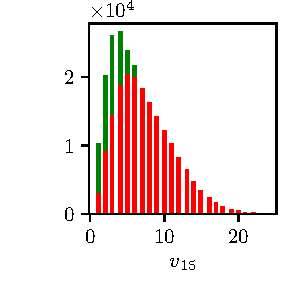
\includegraphics[width=0.241\linewidth]{fig/addendums/pi0_v15}}
\caption{Feature distributions for MVA training of $\pi^0$ candidates in the scope of ROE clean-up.}
\end{figure}

\begin{figure}[H]\ContinuedFloat
\captionsetup{width=0.8\linewidth}
\subfigure{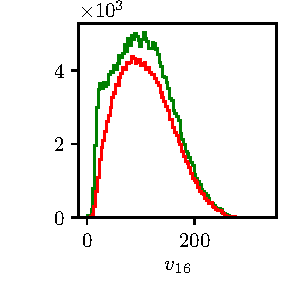
\includegraphics[width=0.241\linewidth]{fig/addendums/pi0_v16}}
\subfigure{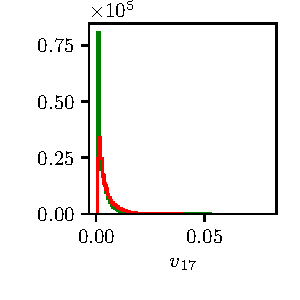
\includegraphics[width=0.241\linewidth]{fig/addendums/pi0_v17}}
\subfigure{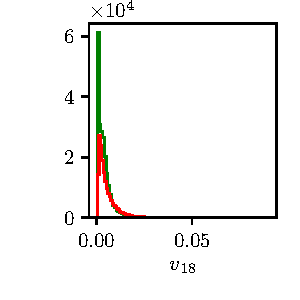
\includegraphics[width=0.241\linewidth]{fig/addendums/pi0_v18}}
\subfigure{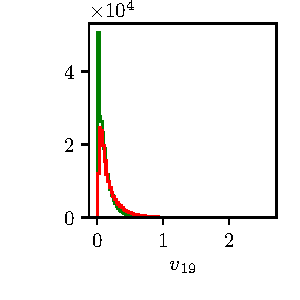
\includegraphics[width=0.241\linewidth]{fig/addendums/pi0_v19}}\\
\subfigure{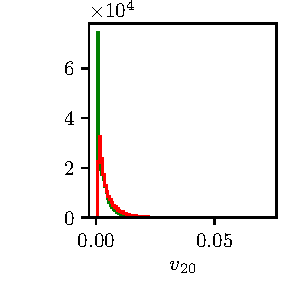
\includegraphics[width=0.241\linewidth]{fig/addendums/pi0_v20}}
\subfigure{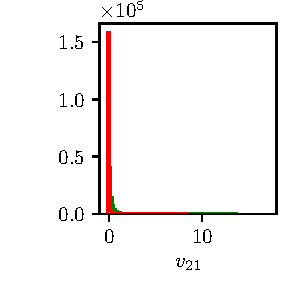
\includegraphics[width=0.241\linewidth]{fig/addendums/pi0_v21}}
\subfigure{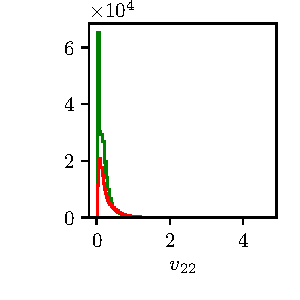
\includegraphics[width=0.241\linewidth]{fig/addendums/pi0_v22}}
\subfigure{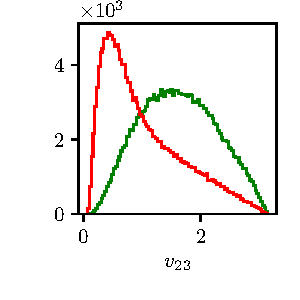
\includegraphics[width=0.241\linewidth]{fig/addendums/pi0_v23}}\\
\subfigure{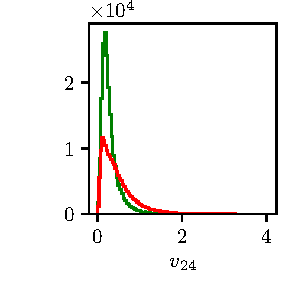
\includegraphics[width=0.241\linewidth]{fig/addendums/pi0_v24}}
\caption{Feature distributions for MVA training of $\pi^0$ candidates in the scope of ROE clean-up.}
\end{figure}

\subsection*{Hyper-parameter optimization}

\begin{figure}[H]
\centering
\captionsetup{width=0.8\linewidth}
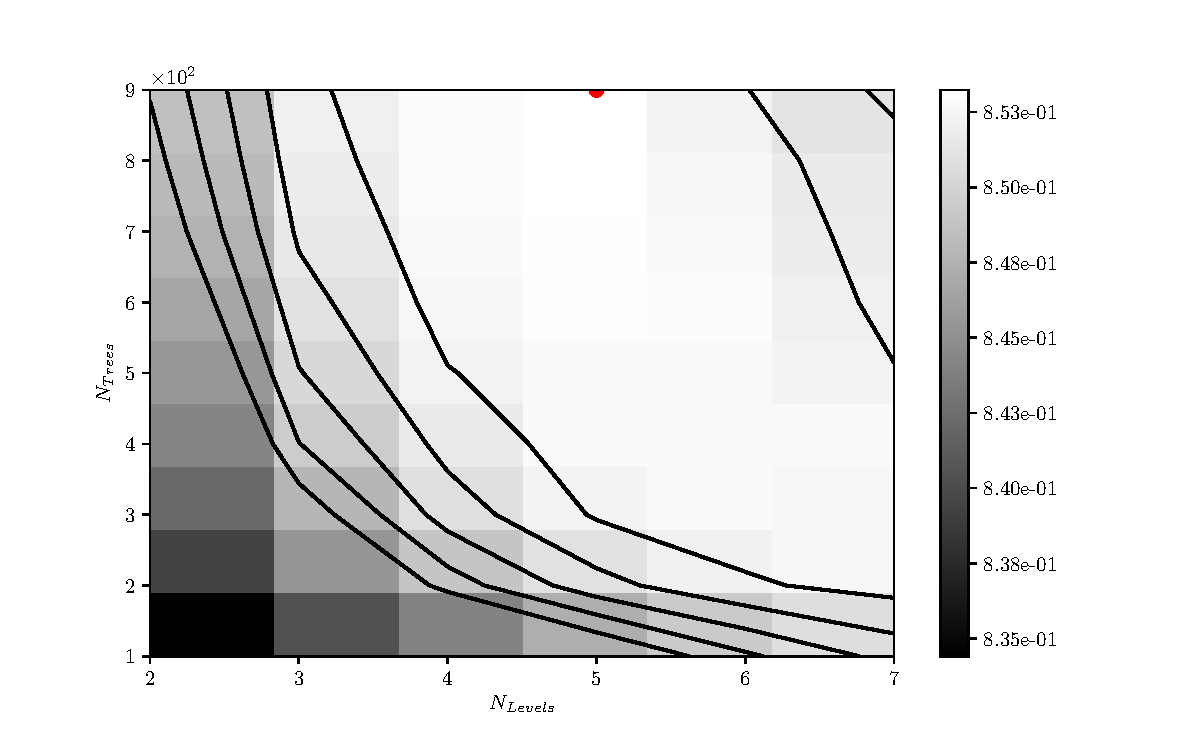
\includegraphics[width=\linewidth]{fig/addendums/pi0_hpo}
\caption{Hyper-parameter optimization of \texttt{nTrees} and \texttt{nLevels} in the BDT forest training of $\pi^0$ candidates in the scope of the ROE clean-up.}
\end{figure}

\subsection*{Results}

\begin{figure}[H]
\centering
\captionsetup{width=0.8\linewidth}
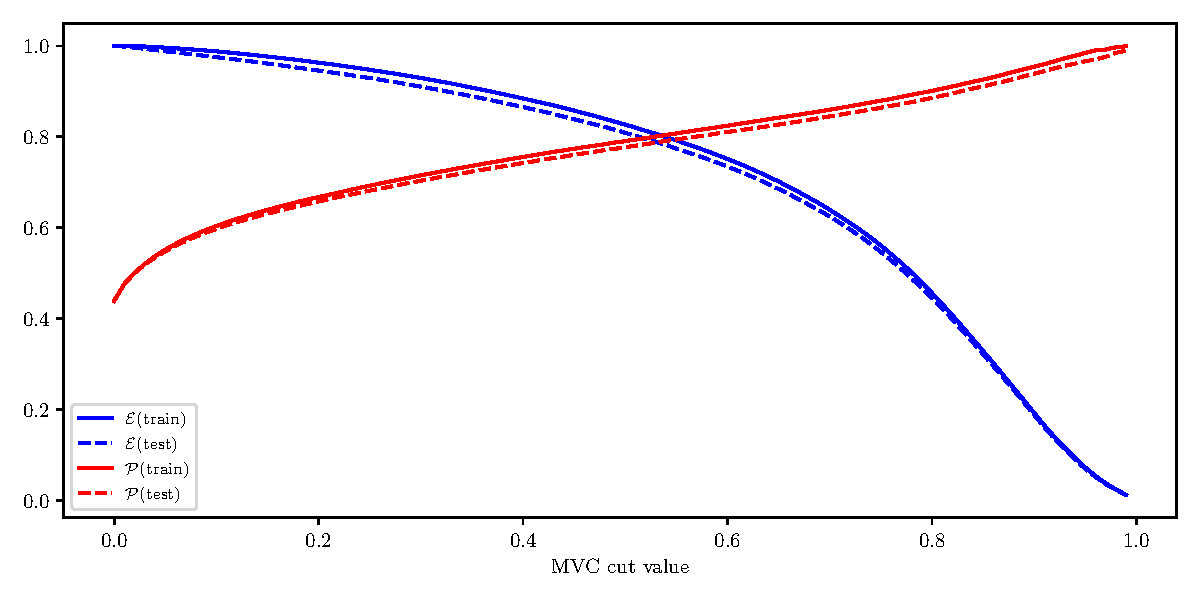
\includegraphics[width=\linewidth]{fig/addendums/pi0_effpur}
\caption{Efficiency ($\mathcal{E}$) and purity ($\mathcal{P}$) of the MVA classifier output for $\pi^0$ candidates training on the train (solid) and test (dashed) samples.}
\end{figure}

\begin{figure}[H]
\centering
\captionsetup{width=0.8\linewidth}
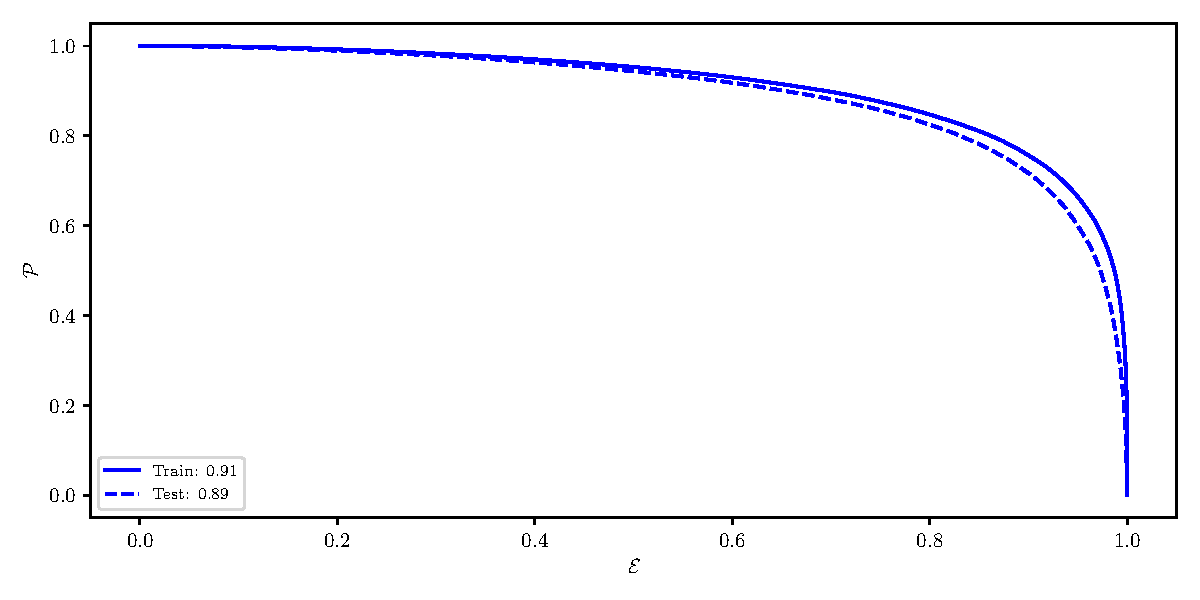
\includegraphics[width=\linewidth]{fig/addendums/pi0_roc}
\caption{ROC curves of the MVA classifier output for $\pi^0$ candidates training on the train (solid) and test (dashed) samples.}
\end{figure}

\section*{ROE clean-up $\gamma$ training}\label{sec:ROE_gamma}

\subsection*{Variable importance}

\begin{longtable}{| p{.05\textwidth} | p{.6\textwidth} | p{.05\textwidth} |p{.2\textwidth} |}
\hline
& Name & Alias & Importance \\ \hline
0 &\texttt{p} & $v_{0}$ & $0.317$ \\ \hline
1 &\texttt{clusterHighestE} & $v_{1}$ & $0.251$ \\ \hline
2 &\texttt{pi0p} & $v_{2}$ & $0.183$ \\ \hline
3 &\texttt{minC2HDist} & $v_{3}$ & $0.058$ \\ \hline
4 &\texttt{cosTheta} & $v_{4}$ & $0.044$ \\ \hline
5 &\texttt{clusterNHits} & $v_{5}$ & $0.031$ \\ \hline
6 &\texttt{clusterE9E25} & $v_{6}$ & $0.030$ \\ \hline
7 &\texttt{useCMSFrame(p)} & $v_{7}$ & $0.028$ \\ \hline
8 &\texttt{clusterUncorrE} & $v_{8}$ & $0.023$ \\ \hline
9 &\texttt{clusterR} & $v_{9}$ & $0.019$ \\ \hline
10 &\texttt{clusterErrorE} & $v_{10}$ & $0.011$ \\ \hline
11 &\texttt{clusterReg} & $v_{11}$ & $0.006$ \\ \hline
\captionsetup{width=0.8\linewidth}
\caption{Variable names, aliases and importance in the scope of $\gamma$ MVA training for ROE clean-up.}
\end{longtable}

\subsection*{Variable distributions}

\begin{figure}[H]
\centering
\captionsetup{width=0.8\linewidth}
\subfigure{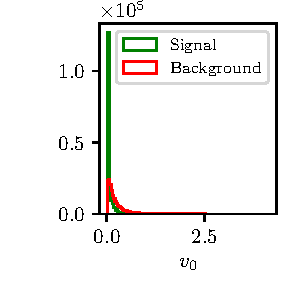
\includegraphics[width=0.241\linewidth]{fig/addendums/gamma_v0}}
\subfigure{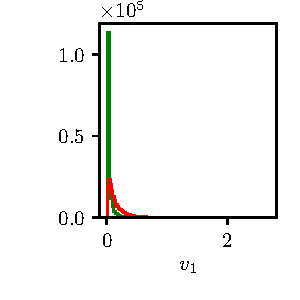
\includegraphics[width=0.241\linewidth]{fig/addendums/gamma_v1}}
\subfigure{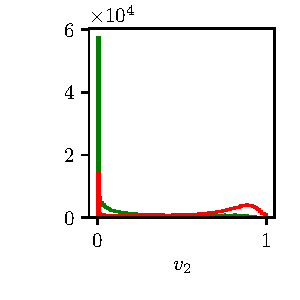
\includegraphics[width=0.241\linewidth]{fig/addendums/gamma_v2}}
\subfigure{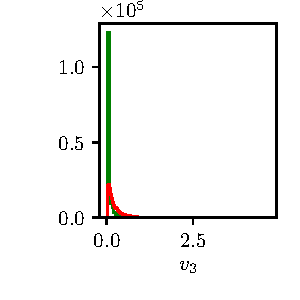
\includegraphics[width=0.241\linewidth]{fig/addendums/gamma_v3}}\\
\subfigure{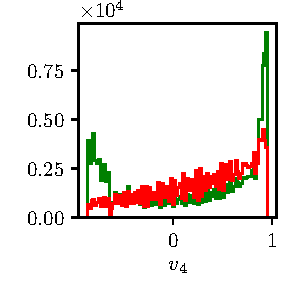
\includegraphics[width=0.241\linewidth]{fig/addendums/gamma_v4}}
\subfigure{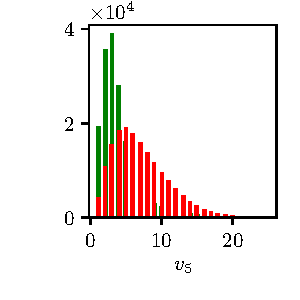
\includegraphics[width=0.241\linewidth]{fig/addendums/gamma_v5}}
\subfigure{\includegraphics[width=0.241\linewidth]{fig/addendums/gamma_v6}}
\subfigure{\includegraphics[width=0.241\linewidth]{fig/addendums/gamma_v7}}\\
\subfigure{\includegraphics[width=0.241\linewidth]{fig/addendums/gamma_v8}}
\subfigure{\includegraphics[width=0.241\linewidth]{fig/addendums/gamma_v9}}
\subfigure{\includegraphics[width=0.241\linewidth]{fig/addendums/gamma_v10}}
\subfigure{\includegraphics[width=0.241\linewidth]{fig/addendums/gamma_v11}}\\
\caption{Feature distributions for MVA training of $\gamma$ candidates in the scope of ROE clean-up.}
\end{figure}

\subsection*{Hyper-parameter optimization}

\begin{figure}[H]
\centering
\captionsetup{width=0.8\linewidth}
\includegraphics[width=\linewidth]{fig/addendums/gamma_hpo}
\caption{Hyper-parameter optimization of \texttt{nTrees} and \texttt{nLevels} in the BDT forest training of $\gamma$ candidates in the scope of the ROE clean-up.}
\end{figure}

\subsection*{Results}

\begin{figure}[H]
\centering
\captionsetup{width=0.8\linewidth}
\includegraphics[width=\linewidth]{fig/addendums/gamma_effpur}
\caption{Efficiency ($\mathcal{E}$) and purity ($\mathcal{P}$) of the MVA classifier output for $\gamma$ candidates training on the train (solid) and test (dashed) samples.}
\end{figure}

\begin{figure}[H]
\centering
\captionsetup{width=0.8\linewidth}
\includegraphics[width=\linewidth]{fig/addendums/gamma_roc}
\caption{ROC curves of the MVA classifier output for $\gamma$ candidates training on the train (solid) and test (dashed) samples.}
\end{figure}

\section*{ROE clean-up duplicate pair training}\label{sec:ROE_dup}

\subsection*{Variable importance}

\begin{longtable}{| p{.05\textwidth} | p{.6\textwidth} | p{.05\textwidth} |p{.2\textwidth} |}
\hline
& Name & Alias & Importance \\ \hline
0 &\texttt{useCMSFrame(daughterAngleInBetween(0,1))} & $v_{0}$ & $0.140$ \\ \hline
1 &\texttt{daughter(1,d0Err)} & $v_{1}$ & $0.084$ \\ \hline
2 &\texttt{useLabFrame(daughterAngleInBetween(0,1))} & $v_{2}$ & $0.056$ \\ \hline
3 &\texttt{daughter(1,d0)} & $v_{3}$ & $0.048$ \\ \hline
4 &\texttt{daughter(0,d0)} & $v_{4}$ & $0.047$ \\ \hline
5 &\texttt{daughter(0,nSVDHits)} & $v_{5}$ & $0.045$ \\ \hline
6 &\texttt{daughter(1,phi0Err)} & $v_{6}$ & $0.042$ \\ \hline
7 &\texttt{daughter(1,nCDCHits)} & $v_{7}$ & $0.038$ \\ \hline
8 &\texttt{daughter(1,z0)} & $v_{8}$ & $0.035$ \\ \hline
9 &\texttt{daughter(0,nCDCHits)} & $v_{9}$ & $0.032$ \\ \hline
10 &\texttt{daughter(0,z0)} & $v_{10}$ & $0.030$ \\ \hline
11 &\texttt{daughter(1,useCMSFrame(p))} & $v_{11}$ & $0.030$ \\ \hline
12 &\texttt{daughter(1,pz)} & $v_{12}$ & $0.026$ \\ \hline
13 &\texttt{extraInfo(decayModeID)} & $v_{13}$ & $0.026$ \\ \hline
14 &\texttt{daughter(0,pz)} & $v_{14}$ & $0.022$ \\ \hline
15 &\texttt{daughter(0,pValue)} & $v_{15}$ & $0.021$ \\ \hline
16 &\texttt{daughter(1,tanlambda)} & $v_{16}$ & $0.021$ \\ \hline
17 &\texttt{daughter(0,d0Err)} & $v_{17}$ & $0.020$ \\ \hline
18 &\texttt{daughter(1,pValue)} & $v_{18}$ & $0.019$ \\ \hline
19 &\texttt{daughter(0,phi0Err)} & $v_{19}$ & $0.018$ \\ \hline
20 &\texttt{daughter(0,useCMSFrame(p))} & $v_{20}$ & $0.018$ \\ \hline
21 &\texttt{daughter(0,tanlambda)} & $v_{21}$ & $0.017$ \\ \hline
22 &\texttt{daughter(0,phi0)} & $v_{22}$ & $0.017$ \\ \hline
23 &\texttt{daughter(1,phi0)} & $v_{23}$ & $0.016$ \\ \hline
24 &\texttt{daughter(0,z0Err)} & $v_{24}$ & $0.014$ \\ \hline
25 &\texttt{daughter(1,omega)} & $v_{25}$ & $0.014$ \\ \hline
26 &\texttt{daughter(0,omega)} & $v_{26}$ & $0.013$ \\ \hline
27 &\texttt{daughter(1,z0Err)} & $v_{27}$ & $0.013$ \\ \hline
28 &\texttt{daughter(0,pt)} & $v_{28}$ & $0.012$ \\ \hline
29 &\texttt{daughter(0,omegaErr)} & $v_{29}$ & $0.012$ \\ \hline
30 &\texttt{daughter(1,pt)} & $v_{30}$ & $0.011$ \\ \hline
31 &\texttt{daughter(1,omegaErr)} & $v_{31}$ & $0.011$ \\ \hline
32 &\texttt{daughter(0,tanlambdaErr)} & $v_{32}$ & $0.010$ \\ \hline
33 &\texttt{daughter(1,nSVDHits)} & $v_{33}$ & $0.010$ \\ \hline
34 &\texttt{daughter(1,tanlambdaErr)} & $v_{34}$ & $0.009$ \\ \hline
35 &\texttt{useRestFrame(daughterAngleInBetween(0,1))} & $v_{35}$ & $0.002$ \\ \hline
36 &\texttt{daughter(1,charge)} & $v_{36}$ & $0.000$ \\ \hline
37 &\texttt{daughter(0,charge)} & $v_{37}$ & $0.000$ \\ \hline
\captionsetup{width=0.8\linewidth}
\caption{Variable names, aliases and importance in the scope of duplicate track pair MVA training for ROE clean-up.}
\end{longtable}

\subsection*{Variable distributions}

\begin{figure}[H]
\centering
\captionsetup{width=0.8\linewidth}
\subfigure{\includegraphics[width=0.241\linewidth]{fig/addendums/dup_v0}}
\subfigure{\includegraphics[width=0.241\linewidth]{fig/addendums/dup_v1}}
\subfigure{\includegraphics[width=0.241\linewidth]{fig/addendums/dup_v2}}
\subfigure{\includegraphics[width=0.241\linewidth]{fig/addendums/dup_v3}}\\
\subfigure{\includegraphics[width=0.241\linewidth]{fig/addendums/dup_v4}}
\subfigure{\includegraphics[width=0.241\linewidth]{fig/addendums/dup_v5}}
\subfigure{\includegraphics[width=0.241\linewidth]{fig/addendums/dup_v6}}
\subfigure{\includegraphics[width=0.241\linewidth]{fig/addendums/dup_v7}}\\
\subfigure{\includegraphics[width=0.241\linewidth]{fig/addendums/dup_v8}}
\subfigure{\includegraphics[width=0.241\linewidth]{fig/addendums/dup_v9}}
\subfigure{\includegraphics[width=0.241\linewidth]{fig/addendums/dup_v10}}
\subfigure{\includegraphics[width=0.241\linewidth]{fig/addendums/dup_v11}}\\
\subfigure{\includegraphics[width=0.241\linewidth]{fig/addendums/dup_v12}}
\subfigure{\includegraphics[width=0.241\linewidth]{fig/addendums/dup_v13}}
\subfigure{\includegraphics[width=0.241\linewidth]{fig/addendums/dup_v14}}
\subfigure{\includegraphics[width=0.241\linewidth]{fig/addendums/dup_v15}}\\
\subfigure{\includegraphics[width=0.241\linewidth]{fig/addendums/dup_v16}}
\subfigure{\includegraphics[width=0.241\linewidth]{fig/addendums/dup_v17}}
\subfigure{\includegraphics[width=0.241\linewidth]{fig/addendums/dup_v18}}
\subfigure{\includegraphics[width=0.241\linewidth]{fig/addendums/dup_v19}}
\caption{Feature distributions for MVA training of duplicate track pair candidates in the scope of ROE clean-up.}
\end{figure}

\begin{figure}[H]\ContinuedFloat
\captionsetup{width=0.8\linewidth}
\subfigure{\includegraphics[width=0.241\linewidth]{fig/addendums/dup_v20}}
\subfigure{\includegraphics[width=0.241\linewidth]{fig/addendums/dup_v21}}
\subfigure{\includegraphics[width=0.241\linewidth]{fig/addendums/dup_v22}}
\subfigure{\includegraphics[width=0.241\linewidth]{fig/addendums/dup_v23}}\\
\subfigure{\includegraphics[width=0.241\linewidth]{fig/addendums/dup_v24}}
\subfigure{\includegraphics[width=0.241\linewidth]{fig/addendums/dup_v25}}
\subfigure{\includegraphics[width=0.241\linewidth]{fig/addendums/dup_v26}}
\subfigure{\includegraphics[width=0.241\linewidth]{fig/addendums/dup_v27}}\\
\subfigure{\includegraphics[width=0.241\linewidth]{fig/addendums/dup_v28}}
\subfigure{\includegraphics[width=0.241\linewidth]{fig/addendums/dup_v29}}
\subfigure{\includegraphics[width=0.241\linewidth]{fig/addendums/dup_v30}}
\subfigure{\includegraphics[width=0.241\linewidth]{fig/addendums/dup_v31}}\\
\subfigure{\includegraphics[width=0.241\linewidth]{fig/addendums/dup_v32}}
\subfigure{\includegraphics[width=0.241\linewidth]{fig/addendums/dup_v33}}
\subfigure{\includegraphics[width=0.241\linewidth]{fig/addendums/dup_v34}}
\subfigure{\includegraphics[width=0.241\linewidth]{fig/addendums/dup_v35}}\\
\subfigure{\includegraphics[width=0.241\linewidth]{fig/addendums/dup_v36}}
\subfigure{\includegraphics[width=0.241\linewidth]{fig/addendums/dup_v37}}
\caption{Feature distributions for MVA training of duplicate track pair candidates in the scope of ROE clean-up.}
\end{figure}

\subsection*{Hyper-parameter optimization}

\begin{figure}[H]
\centering
\captionsetup{width=0.8\linewidth}
\includegraphics[width=\linewidth]{fig/addendums/dup_hpo}
\caption{Hyper-parameter optimization of \texttt{nTrees} and \texttt{nLevels} in the BDT forest training of duplicate track pair candidates in the scope of the ROE clean-up.}
\end{figure}

\subsection*{Results}

\begin{figure}[H]
\centering
\captionsetup{width=0.8\linewidth}
\includegraphics[width=\linewidth]{fig/addendums/dup_effpur}
\caption{Efficiency ($\mathcal{E}$) and purity ($\mathcal{P}$) of the MVA classifier output for duplicate track pair candidates training on the train (solid) and test (dashed) samples.}
\end{figure}

\begin{figure}[H]
\centering
\captionsetup{width=0.8\linewidth}
\includegraphics[width=\linewidth]{fig/addendums/dup_roc}
\caption{ROC curves of the MVA classifier output for duplicate track pair candidates training on the train (solid) and test (dashed) samples.}
\end{figure}

\section*{ROE clean-up duplicate track training}\label{sec:ROE_curl}

\subsection*{Variable importance}

\begin{longtable}{| p{.05\textwidth} | p{.6\textwidth} | p{.05\textwidth} |p{.2\textwidth} |}
\hline
& Name & Alias & Importance \\ \hline
0 &\texttt{d0} & $v_{0}$ & $0.093$ \\ \hline
1 &\texttt{extraInfo(nSVDHitsDiff)} & $v_{1}$ & $0.089$ \\ \hline
2 &\texttt{z0} & $v_{2}$ & $0.080$ \\ \hline
3 &\texttt{extraInfo(pValueDiff)} & $v_{3}$ & $0.060$ \\ \hline
4 &\texttt{extraInfo(ptDiff)} & $v_{4}$ & $0.059$ \\ \hline
5 &\texttt{extraInfo(z0Diff)} & $v_{5}$ & $0.055$ \\ \hline
6 &\texttt{extraInfo(phi0Diff)} & $v_{6}$ & $0.046$ \\ \hline
7 &\texttt{extraInfo(pzDiff)} & $v_{7}$ & $0.045$ \\ \hline
8 &\texttt{extraInfo(nCDCHitsDiff)} & $v_{8}$ & $0.043$ \\ \hline
9 &\texttt{phi0Err} & $v_{9}$ & $0.042$ \\ \hline
10 &\texttt{extraInfo(tanlambdaDiff)} & $v_{10}$ & $0.039$ \\ \hline
11 &\texttt{z0Err} & $v_{11}$ & $0.035$ \\ \hline
12 &\texttt{pValue} & $v_{12}$ & $0.030$ \\ \hline
13 &\texttt{extraInfo(omegaDiff)} & $v_{13}$ & $0.030$ \\ \hline
14 &\texttt{tanlambdaErr} & $v_{14}$ & $0.029$ \\ \hline
15 &\texttt{nCDCHits} & $v_{15}$ & $0.028$ \\ \hline
16 &\texttt{pt} & $v_{16}$ & $0.027$ \\ \hline
17 &\texttt{d0Err} & $v_{17}$ & $0.025$ \\ \hline
18 &\texttt{phi0} & $v_{18}$ & $0.025$ \\ \hline
19 &\texttt{pz} & $v_{19}$ & $0.024$ \\ \hline
20 &\texttt{cosTheta} & $v_{20}$ & $0.022$ \\ \hline
21 &\texttt{omegaErr} & $v_{21}$ & $0.022$ \\ \hline
22 &\texttt{useCMSFrame(p)} & $v_{22}$ & $0.021$ \\ \hline
23 &\texttt{omega} & $v_{23}$ & $0.018$ \\ \hline
24 &\texttt{nSVDHits} & $v_{24}$ & $0.014$ \\ \hline
\captionsetup{width=0.8\linewidth}
\caption{Variable names, aliases and importance in the scope of duplicate track MVA training for ROE clean-up.}
\end{longtable}

\subsection*{Variable distributions}

\begin{figure}[H]
\centering
\captionsetup{width=0.8\linewidth}
\subfigure{\includegraphics[width=0.241\linewidth]{fig/addendums/curl_v0}}
\subfigure{\includegraphics[width=0.241\linewidth]{fig/addendums/curl_v1}}
\subfigure{\includegraphics[width=0.241\linewidth]{fig/addendums/curl_v2}}
\subfigure{\includegraphics[width=0.241\linewidth]{fig/addendums/curl_v3}}\\
\subfigure{\includegraphics[width=0.241\linewidth]{fig/addendums/curl_v4}}
\subfigure{\includegraphics[width=0.241\linewidth]{fig/addendums/curl_v5}}
\subfigure{\includegraphics[width=0.241\linewidth]{fig/addendums/curl_v6}}
\subfigure{\includegraphics[width=0.241\linewidth]{fig/addendums/curl_v7}}\\
\subfigure{\includegraphics[width=0.241\linewidth]{fig/addendums/curl_v8}}
\subfigure{\includegraphics[width=0.241\linewidth]{fig/addendums/curl_v9}}
\subfigure{\includegraphics[width=0.241\linewidth]{fig/addendums/curl_v10}}
\subfigure{\includegraphics[width=0.241\linewidth]{fig/addendums/curl_v11}}\\
\subfigure{\includegraphics[width=0.241\linewidth]{fig/addendums/curl_v12}}
\subfigure{\includegraphics[width=0.241\linewidth]{fig/addendums/curl_v13}}
\subfigure{\includegraphics[width=0.241\linewidth]{fig/addendums/curl_v14}}
\subfigure{\includegraphics[width=0.241\linewidth]{fig/addendums/curl_v15}}\\
\subfigure{\includegraphics[width=0.241\linewidth]{fig/addendums/curl_v16}}
\subfigure{\includegraphics[width=0.241\linewidth]{fig/addendums/curl_v17}}
\subfigure{\includegraphics[width=0.241\linewidth]{fig/addendums/curl_v18}}
\subfigure{\includegraphics[width=0.241\linewidth]{fig/addendums/curl_v19}}
\caption{Feature distributions for MVA training of duplicate track candidates in the scope of ROE clean-up.}
\end{figure}

\begin{figure}[H]\ContinuedFloat
\captionsetup{width=0.8\linewidth}
\subfigure{\includegraphics[width=0.241\linewidth]{fig/addendums/curl_v20}}
\subfigure{\includegraphics[width=0.241\linewidth]{fig/addendums/curl_v21}}
\subfigure{\includegraphics[width=0.241\linewidth]{fig/addendums/curl_v22}}
\subfigure{\includegraphics[width=0.241\linewidth]{fig/addendums/curl_v23}}\\
\subfigure{\includegraphics[width=0.241\linewidth]{fig/addendums/curl_v24}}
\caption{Feature distributions for MVA training of duplicate track candidates in the scope of ROE clean-up.}
\end{figure}

\subsection*{Hyper-parameter optimization}

\begin{figure}[H]
\centering
\captionsetup{width=0.8\linewidth}
\includegraphics[width=\linewidth]{fig/addendums/curl_hpo}
\caption{Hyper-parameter optimization of \texttt{nTrees} and \texttt{nLevels} in the BDT forest training of duplicate track candidates in the scope of the ROE clean-up.}
\end{figure}

\subsection*{Results}

\begin{figure}[H]
\centering
\captionsetup{width=0.8\linewidth}
\includegraphics[width=\linewidth]{fig/addendums/curl_effpur}
\caption{Efficiency ($\mathcal{E}$) and purity ($\mathcal{P}$) of the MVA classifier output for duplicate track candidates training on the train (solid) and test (dashed) samples.}
\end{figure}

\begin{figure}[H]
\centering
\captionsetup{width=0.8\linewidth}
\includegraphics[width=\linewidth]{fig/addendums/curl_roc}
\caption{ROC curves of the MVA classifier output for duplicate track candidates training on the train (solid) and test (dashed) samples.}
\end{figure}

\section*{$q \bar q$ suppression training}

\subsection*{Variable importance}

\begin{longtable}{| p{.05\textwidth} | p{.6\textwidth} | p{.05\textwidth} |p{.2\textwidth} |}
\hline
& Name & Alias & Importance \\ \hline
0 &\texttt{B\_R2} & $v_{0}$ & $0.275$ \\ \hline
1 &\texttt{B\_CosTBTO} & $v_{1}$ & $0.162$ \\ \hline
2 &\texttt{B\_ThrustB} & $v_{2}$ & $0.066$ \\ \hline
3 &\texttt{B\_roeFit\_dz} & $v_{3}$ & $0.056$ \\ \hline
4 &\texttt{B\_hso02} & $v_{4}$ & $0.056$ \\ \hline
5 &\texttt{B\_ThrustO} & $v_{5}$ & $0.035$ \\ \hline
6 &\texttt{B\_hoo2} & $v_{6}$ & $0.034$ \\ \hline
7 &\texttt{B\_hso12} & $v_{7}$ & $0.025$ \\ \hline
8 &\texttt{B\_qpFastHadron} & $v_{8}$ & $0.020$ \\ \hline
9 &\texttt{B\_hoo0} & $v_{9}$ & $0.018$ \\ \hline
10 &\texttt{B\_cc2\_CcROE} & $v_{10}$ & $0.018$ \\ \hline
11 &\texttt{B\_CosTBz} & $v_{11}$ & $0.017$ \\ \hline
12 &\texttt{B\_qpKaon} & $v_{12}$ & $0.016$ \\ \hline
13 &\texttt{B\_cc3\_CcROE} & $v_{13}$ & $0.016$ \\ \hline
14 &\texttt{B\_hso01} & $v_{14}$ & $0.016$ \\ \hline
15 &\texttt{B\_cc4\_CcROE} & $v_{15}$ & $0.015$ \\ \hline
16 &\texttt{B\_qpMaximumPstar} & $v_{16}$ & $0.014$ \\ \hline
17 &\texttt{B\_cc5\_CcROE} & $v_{17}$ & $0.012$ \\ \hline
18 &\texttt{B\_cc1\_CcROE} & $v_{18}$ & $0.011$ \\ \hline
19 &\texttt{B\_cc6\_CcROE} & $v_{19}$ & $0.011$ \\ \hline
20 &\texttt{B\_cc7\_CcROE} & $v_{20}$ & $0.010$ \\ \hline
21 &\texttt{B\_cc9\_CcROE} & $v_{21}$ & $0.009$ \\ \hline
22 &\texttt{B\_qpSlowPion} & $v_{22}$ & $0.009$ \\ \hline
23 &\texttt{B\_cc8\_CcROE} & $v_{23}$ & $0.009$ \\ \hline
24 &\texttt{B\_qpFSC} & $v_{24}$ & $0.009$ \\ \hline
25 &\texttt{B\_qpLambda} & $v_{25}$ & $0.008$ \\ \hline
26 &\texttt{B\_hoo1} & $v_{26}$ & $0.008$ \\ \hline
27 &\texttt{B\_qpKaonPion} & $v_{27}$ & $0.008$ \\ \hline
28 &\texttt{B\_hso10} & $v_{28}$ & $0.007$ \\ \hline
29 &\texttt{B\_hoo4} & $v_{29}$ & $0.007$ \\ \hline
30 &\texttt{B\_hso04} & $v_{30}$ & $0.006$ \\ \hline
31 &\texttt{B\_hso03} & $v_{31}$ & $0.005$ \\ \hline
32 &\texttt{B\_hoo3} & $v_{32}$ & $0.005$ \\ \hline
33 &\texttt{B\_hso14} & $v_{33}$ & $0.005$ \\ \hline
\captionsetup{width=0.8\linewidth}
\caption{Variable names, aliases and importance in the scope of $q\bar q$ suppression MVA training.}
\end{longtable}

\subsection*{Variable distributions}

\begin{figure}[H]
\centering
\captionsetup{width=0.8\linewidth}
\subfigure{\includegraphics[width=0.241\linewidth]{fig/addendums/QQ_v0}}
\subfigure{\includegraphics[width=0.241\linewidth]{fig/addendums/QQ_v1}}
\subfigure{\includegraphics[width=0.241\linewidth]{fig/addendums/QQ_v2}}
\subfigure{\includegraphics[width=0.241\linewidth]{fig/addendums/QQ_v3}}\\
\subfigure{\includegraphics[width=0.241\linewidth]{fig/addendums/QQ_v4}}
\subfigure{\includegraphics[width=0.241\linewidth]{fig/addendums/QQ_v5}}
\subfigure{\includegraphics[width=0.241\linewidth]{fig/addendums/QQ_v6}}
\subfigure{\includegraphics[width=0.241\linewidth]{fig/addendums/QQ_v7}}\\
\subfigure{\includegraphics[width=0.241\linewidth]{fig/addendums/QQ_v8}}
\subfigure{\includegraphics[width=0.241\linewidth]{fig/addendums/QQ_v9}}
\subfigure{\includegraphics[width=0.241\linewidth]{fig/addendums/QQ_v10}}
\subfigure{\includegraphics[width=0.241\linewidth]{fig/addendums/QQ_v11}}\\
\subfigure{\includegraphics[width=0.241\linewidth]{fig/addendums/QQ_v12}}
\subfigure{\includegraphics[width=0.241\linewidth]{fig/addendums/QQ_v13}}
\subfigure{\includegraphics[width=0.241\linewidth]{fig/addendums/QQ_v14}}
\subfigure{\includegraphics[width=0.241\linewidth]{fig/addendums/QQ_v15}}\\
\subfigure{\includegraphics[width=0.241\linewidth]{fig/addendums/QQ_v16}}
\subfigure{\includegraphics[width=0.241\linewidth]{fig/addendums/QQ_v17}}
\subfigure{\includegraphics[width=0.241\linewidth]{fig/addendums/QQ_v18}}
\subfigure{\includegraphics[width=0.241\linewidth]{fig/addendums/QQ_v19}}
\caption{Feature distributions for MVA training of $q\bar q$ background suppression.}
\end{figure}

\begin{figure}[H]\ContinuedFloat
\captionsetup{width=0.8\linewidth}
\subfigure{\includegraphics[width=0.241\linewidth]{fig/addendums/QQ_v20}}
\subfigure{\includegraphics[width=0.241\linewidth]{fig/addendums/QQ_v21}}
\subfigure{\includegraphics[width=0.241\linewidth]{fig/addendums/QQ_v22}}
\subfigure{\includegraphics[width=0.241\linewidth]{fig/addendums/QQ_v23}}\\
\subfigure{\includegraphics[width=0.241\linewidth]{fig/addendums/QQ_v24}}
\subfigure{\includegraphics[width=0.241\linewidth]{fig/addendums/QQ_v25}}
\subfigure{\includegraphics[width=0.241\linewidth]{fig/addendums/QQ_v26}}
\subfigure{\includegraphics[width=0.241\linewidth]{fig/addendums/QQ_v27}}\\
\subfigure{\includegraphics[width=0.241\linewidth]{fig/addendums/QQ_v28}}
\subfigure{\includegraphics[width=0.241\linewidth]{fig/addendums/QQ_v29}}
\subfigure{\includegraphics[width=0.241\linewidth]{fig/addendums/QQ_v30}}
\subfigure{\includegraphics[width=0.241\linewidth]{fig/addendums/QQ_v31}}\\
\subfigure{\includegraphics[width=0.241\linewidth]{fig/addendums/QQ_v32}}
\subfigure{\includegraphics[width=0.241\linewidth]{fig/addendums/QQ_v33}}
\caption{Feature distributions for MVA training of $q\bar q$ background suppression.}
\end{figure}

\subsection*{Hyper-parameter optimization}

\begin{figure}[H]
\centering
\captionsetup{width=0.8\linewidth}
\includegraphics[width=\linewidth]{fig/addendums/QQ_hpo}
\caption{Hyper-parameter optimization of \texttt{nTrees} and \texttt{nLevels} in the BDT forest training of $q\bar q$ background suppression.}
\end{figure}

\subsection*{Results}

\begin{figure}[H]
\centering
\captionsetup{width=0.8\linewidth}
\includegraphics[width=\linewidth]{fig/addendums/QQ_effpur}
\caption{Efficiency ($\mathcal{E}$) and purity ($\mathcal{P}$) of the MVA classifier output for $q\bar q$ background suppression training on the train (solid) and test (dashed) samples.}
\end{figure}

\begin{figure}[H]
\centering
\captionsetup{width=0.8\linewidth}
\includegraphics[width=\linewidth]{fig/addendums/QQ_roc}
\caption{ROC curves of the MVA classifier output for $q\bar q$ background suppression training on the train (solid) and test (dashed) samples.}
\end{figure}

\section*{Standard $B \bar B$ suppression training}

\subsection*{Variable importance}

\begin{longtable}{| p{.05\textwidth} | p{.6\textwidth} | p{.05\textwidth} |p{.2\textwidth} |}
\hline
& Name & Alias & Importance \\ \hline
0 &\texttt{B\_cosMomVtxKKlnu} & $v_{0}$ & $0.412$ \\ \hline
1 &\texttt{B\_ROE\_PThetacms0} & $v_{1}$ & $0.101$ \\ \hline
2 &\texttt{B\_nROETrk0} & $v_{2}$ & $0.067$ \\ \hline
3 &\texttt{B\_K1FT} & $v_{3}$ & $0.056$ \\ \hline
4 &\texttt{B\_nROEDistTrk} & $v_{4}$ & $0.055$ \\ \hline
5 &\texttt{B\_cosBY} & $v_{5}$ & $0.042$ \\ \hline
6 &\texttt{B\_xiZ0} & $v_{6}$ & $0.038$ \\ \hline
7 &\texttt{B\_roeFit\_dz} & $v_{7}$ & $0.034$ \\ \hline
8 &\texttt{B\_cosMomVtx} & $v_{8}$ & $0.033$ \\ \hline
9 &\texttt{B\_missM2Veto1} & $v_{9}$ & $0.030$ \\ \hline
10 &\texttt{B\_nKaonInROE} & $v_{10}$ & $0.021$ \\ \hline
11 &\texttt{B\_QVeto1} & $v_{11}$ & $0.020$ \\ \hline
12 &\texttt{B\_chiProb} & $v_{12}$ & $0.017$ \\ \hline
13 &\texttt{B\_K0FT} & $v_{13}$ & $0.016$ \\ \hline
14 &\texttt{B\_TagVPvalue} & $v_{14}$ & $0.015$ \\ \hline
15 &\texttt{B\_cosMomVtxKK} & $v_{15}$ & $0.014$ \\ \hline
16 &\texttt{B\_missM20} & $v_{16}$ & $0.014$ \\ \hline
17 &\texttt{B\_missM2Veto2} & $v_{17}$ & $0.007$ \\ \hline
18 &\texttt{B\_QVeto2} & $v_{18}$ & $0.006$ \\ \hline
\captionsetup{width=0.8\linewidth}
\caption{Variable names, aliases and importance in the scope of $B\bar B$ background suppression.}
\end{longtable}

\subsection*{Variable distributions}

\begin{figure}[H]
\centering
\captionsetup{width=0.8\linewidth}
\subfigure{\includegraphics[width=0.241\linewidth]{fig/addendums/BB01c_v0}}
\subfigure{\includegraphics[width=0.241\linewidth]{fig/addendums/BB01c_v1}}
\subfigure{\includegraphics[width=0.241\linewidth]{fig/addendums/BB01c_v2}}
\subfigure{\includegraphics[width=0.241\linewidth]{fig/addendums/BB01c_v3}}\\
\subfigure{\includegraphics[width=0.241\linewidth]{fig/addendums/BB01c_v4}}
\subfigure{\includegraphics[width=0.241\linewidth]{fig/addendums/BB01c_v5}}
\subfigure{\includegraphics[width=0.241\linewidth]{fig/addendums/BB01c_v6}}
\subfigure{\includegraphics[width=0.241\linewidth]{fig/addendums/BB01c_v7}}\\
\subfigure{\includegraphics[width=0.241\linewidth]{fig/addendums/BB01c_v8}}
\subfigure{\includegraphics[width=0.241\linewidth]{fig/addendums/BB01c_v9}}
\subfigure{\includegraphics[width=0.241\linewidth]{fig/addendums/BB01c_v10}}
\subfigure{\includegraphics[width=0.241\linewidth]{fig/addendums/BB01c_v11}}\\
\subfigure{\includegraphics[width=0.241\linewidth]{fig/addendums/BB01c_v12}}
\subfigure{\includegraphics[width=0.241\linewidth]{fig/addendums/BB01c_v13}}
\subfigure{\includegraphics[width=0.241\linewidth]{fig/addendums/BB01c_v14}}
\subfigure{\includegraphics[width=0.241\linewidth]{fig/addendums/BB01c_v15}}\\
\subfigure{\includegraphics[width=0.241\linewidth]{fig/addendums/BB01c_v16}}
\subfigure{\includegraphics[width=0.241\linewidth]{fig/addendums/BB01c_v17}}
\subfigure{\includegraphics[width=0.241\linewidth]{fig/addendums/BB01c_v18}}
\caption{Feature distributions for MVA training of $B\bar B$ background suppression.}
\end{figure}

\subsection*{Hyper-parameter optimization}

\begin{figure}[H]
\centering
\captionsetup{width=0.8\linewidth}
\includegraphics[width=\linewidth]{fig/addendums/BB01c_hpo}
\caption{Hyper-parameter optimization of \texttt{nTrees} and \texttt{nLevels} in the BDT forest training of $B\bar B$ background suppression.}
\end{figure}

\subsection*{Results}

\begin{figure}[H]
\centering
\captionsetup{width=0.8\linewidth}
\includegraphics[width=\linewidth]{fig/addendums/BB01c_effpur}
\caption{Efficiency ($\mathcal{E}$) and purity ($\mathcal{P}$) of the MVA classifier output for $B\bar B$ background suppression training on the train (solid) and test (dashed) samples.}
\end{figure}

\begin{figure}[H]
\centering
\captionsetup{width=0.8\linewidth}
\includegraphics[width=\linewidth]{fig/addendums/BB01c_roc}
\caption{ROC curves of the MVA classifier output for $B\bar B$ background suppression training on the train (solid) and test (dashed) samples.}
\end{figure}

\section*{Uniformity boosted $B \bar B$ suppression training}

\subsection*{Hyper-parameter optimization}

Hyper-parameters were not optimized due to the large CPU time consumption of the algorithm. The following set up of the hyper-parameters was chosen
\begin{itemize}
\item \texttt{nTrees}: 300
\item \texttt{nLevels}: 4
\end{itemize}

\subsection*{Results}

\begin{figure}[H]
\centering
\captionsetup{width=0.8\linewidth}
\includegraphics[width=\linewidth]{fig/addendums/uMVA1dc_effpur}
\caption{Efficiency ($\mathcal{E}$) and purity ($\mathcal{P}$) of the uniformity boosted MVA classifier output for $B\bar B$ background suppression training on the train (solid) and test (dashed) samples.}
\end{figure}

\begin{figure}[H]
\centering
\captionsetup{width=0.8\linewidth}
\includegraphics[width=\linewidth]{fig/addendums/uMVA1dc_roc}
\caption{ROC curves of the uniformity boosted MVA classifier output for $B\bar B$ background suppression training on the train (solid) and test (dashed) samples.}
\end{figure}